\section{Technology classification detail}
\label{app:nlp}

\subsection*{Annotated corpus}

500 manually annotated BOAMP notices, 2015--2025, all with a non-empty object text, no duplicate identifiers.
The sample is quota-stratified, so the class shares below are a property of the annotation design and are not
prevalence estimates.

\begin{longtable}[]{@{}lrr@{}}
\toprule\noalign{}
Class & $n$ & Share \\
\midrule\noalign{}
\endhead
BUSINESS\_SOFTWARE & 88 & 0.176 \\
NETWORK\_TELECOM & 81 & 0.162 \\
IT\_SERVICES & 74 & 0.148 \\
CYBERSECURITY & 54 & 0.108 \\
OTHER\_DIGITAL & 53 & 0.106 \\
IT\_INFRASTRUCTURE & 46 & 0.092 \\
CLOUD\_HOSTING & 32 & 0.064 \\
DATA\_BI & 29 & 0.058 \\
MIXED & 21 & 0.042 \\
OTHER & 15 & 0.030 \\
AI & 7 & 0.014 \\
\bottomrule\noalign{}
\end{longtable}

451 of the 500 notices are in the Grand Ouest and all 500 carry a digital CPV; 434 are tender notices, 55
award notices and 9 corrections. Only 243 belong to cohort episodes, so performance measured on this corpus
is evidence about the corpus rather than about the deployment population.

\subsection*{Specification comparison}

All six specifications share identical group-aware folds and an identical inner search budget.

\begingroup
\small
\setlength{\tabcolsep}{4pt}
\begin{longtable}[]{@{}llrr@{}}
\toprule\noalign{}
Model & Features & CV macro-F1 (SD) & Out-of-fold macro-F1 \\
\midrule\noalign{}
\endhead
\texttt{M\_majority} & --- & 0.027 (0.000) & --- \\
\texttt{M0\_cpv} & CPV tokens & 0.439 (0.076) & 0.441 \\
\texttt{M0b\_cpv\_descriptor} & CPV + descriptors & 0.469 (0.038) & 0.473 \\
\texttt{M1\_tfidf\_logreg} & object text & 0.662 (0.067) & 0.670 \\
\textbf{\texttt{M2\_tfidf\_logreg\_balanced}} & object text & \textbf{0.741 (0.034)} & \textbf{0.744} \\
\texttt{M3\_tfidf\_linearsvm} & object text & 0.717 (0.030) & 0.718 \\
\texttt{M4\_tfidf\_linearsvm\_balanced} & object text & 0.716 (0.054) & 0.715 \\
\bottomrule\noalign{}
\end{longtable}
\endgroup

Two aggregations appear above and should not be confused: the CV column averages the three fold scores, while
the out-of-fold column computes one score over the pooled 500 held-out predictions.

\subsection*{Per-class performance, out of fold}

\begin{longtable}[]{@{}lrrrrr@{}}
\toprule\noalign{}
Class & Precision & Recall & F1 & Support & Predicted \\
\midrule\noalign{}
\endhead
DATA\_BI & 0.923 & 0.828 & 0.873 & 29 & 26 \\
OTHER & 0.923 & 0.800 & 0.857 & 15 & 13 \\
BUSINESS\_SOFTWARE & 0.798 & 0.898 & 0.845 & 88 & 99 \\
NETWORK\_TELECOM & 0.810 & 0.840 & 0.824 & 81 & 84 \\
CYBERSECURITY & 0.848 & 0.722 & 0.780 & 54 & 46 \\
IT\_SERVICES & 0.778 & 0.757 & 0.767 & 74 & 72 \\
IT\_INFRASTRUCTURE & 0.702 & 0.717 & 0.710 & 46 & 47 \\
OTHER\_DIGITAL & 0.655 & 0.679 & 0.667 & 53 & 55 \\
AI & 0.800 & 0.571 & \emph{0.667} & \emph{7} & 5 \\
CLOUD\_HOSTING & 0.731 & 0.594 & 0.655 & 32 & 26 \\
MIXED & 0.482 & 0.619 & 0.542 & 21 & 27 \\
\bottomrule\noalign{}
\end{longtable}

The \texttt{AI} row is printed with its support and marked unevaluable: an F1 of 0.667 on seven annotated
notices rests on three correct predictions, and both a high and a low value would be uninformative.

\subsection*{Error triage}

Thirty representative out-of-fold errors were sampled from the largest confusion pairs: 16 model errors,
7 taxonomy-boundary ambiguities, 4 genuinely multi-technology procurements, 2 annotation inconsistencies in
related notices, 1 object text too poor to decide. Close to half the residual therefore comes from class
definitions or missing information rather than from model capacity --- which is also why a larger model was
not the indicated remedy.

\subsection*{Temporal robustness}

Training 2015--2022 ($n = 393$), test 2023--2025 ($n = 107$), with the four boundary-straddling families
assigned to training in full. All-class macro-F1 0.662; macro-F1 over the five classes with test support of
at least 10 (\texttt{CYBERSECURITY}, \texttt{NETWORK\_TELECOM}, \texttt{BUSINESS\_SOFTWARE},
\texttt{IT\_SERVICES}, \texttt{OTHER\_DIGITAL}) is 0.815; weighted F1 0.772; accuracy 0.776.

\subsection*{Deployed confidence: reliability out of fold}

\begin{longtable}[]{@{}lrrrr@{}}
\toprule\noalign{}
Stated confidence & $n$ & Observed accuracy & Mean stated & Gap \\
\midrule\noalign{}
\endhead
$[0.0,0.3)$ & 151 & 0.523 & 0.224 & $+0.299$ \\
$[0.3,0.4)$ & 114 & 0.825 & 0.349 & $+0.476$ \\
$[0.4,0.5)$ & 91 & 0.813 & 0.454 & $+0.359$ \\
$[0.5,0.6)$ & 57 & 0.983 & 0.544 & $+0.438$ \\
$[0.6,0.7)$ & 42 & 0.905 & 0.653 & $+0.252$ \\
$[0.7,0.8)$ & 26 & 0.962 & 0.735 & $+0.227$ \\
$[0.8,0.9)$ & 16 & 0.938 & 0.854 & $+0.084$ \\
$[0.9,1.0)$ & 3 & 1.000 & 0.938 & $+0.062$ \\
\bottomrule\noalign{}
\end{longtable}

The gap is positive in every bin above 0.3: the score understates its own hit rate. Expected calibration
error of the deployed variant is 0.350. Platt scaling cut that error by 0.1405 --- clearing the 0.02
requirement --- but cost 0.0364 macro-F1, exceeding the 0.02 budget, so the pre-specified rule rejected it and
the rule was not relaxed.

Cohort coverage by cutoff: 648 episodes at $\ge 0.5$, 412 at $\ge 0.6$, 235 at $\ge 0.7$, 123 at $\ge 0.8$,
28 at $\ge 0.9$; the highest deployed confidence is 0.9707.

\subsection*{Downstream eligibility}

\begin{longtable}[]{@{}lrrrll@{}}
\toprule\noalign{}
Class & CV F1 & Episodes & Events & Gate A & Gate B \\
\midrule\noalign{}
\endhead
CYBERSECURITY & 0.780 & 316 & 60 & pass & pass \\
NETWORK\_TELECOM & 0.824 & 859 & 140 & pass & pass \\
IT\_INFRASTRUCTURE & 0.710 & 298 & 38 & pass & pass \\
BUSINESS\_SOFTWARE & 0.845 & 854 & 106 & pass & pass \\
IT\_SERVICES & 0.767 & 492 & 72 & pass & pass \\
CLOUD\_HOSTING & 0.655 & 115 & 11 & pass & fail \\
DATA\_BI & 0.873 & 86 & 15 & pass & fail \\
AI & 0.667 & 6 & 0 & fail & fail \\
MIXED & 0.542 & 139 & 32 & fail & pass \\
OTHER\_DIGITAL & 0.667 & 462 & 44 & fail & pass \\
OTHER & 0.857 & 173 & 26 & fail & pass \\
\bottomrule\noalign{}
\end{longtable}

Gate A requires a substantive technology class with annotated support $\ge 10$ and out-of-fold F1 $\ge 0.65$;
Gate B requires $\ge 100$ episodes and $\ge 20$ events. Applying Gate A moves the technology log-rank result
from $p = 0.000119$ (8 classes, 518 events) to $p = 0.0363$ (5 classes, 416 events). The gate costs
significance and was kept.

\begin{figure}[htbp]
\centering
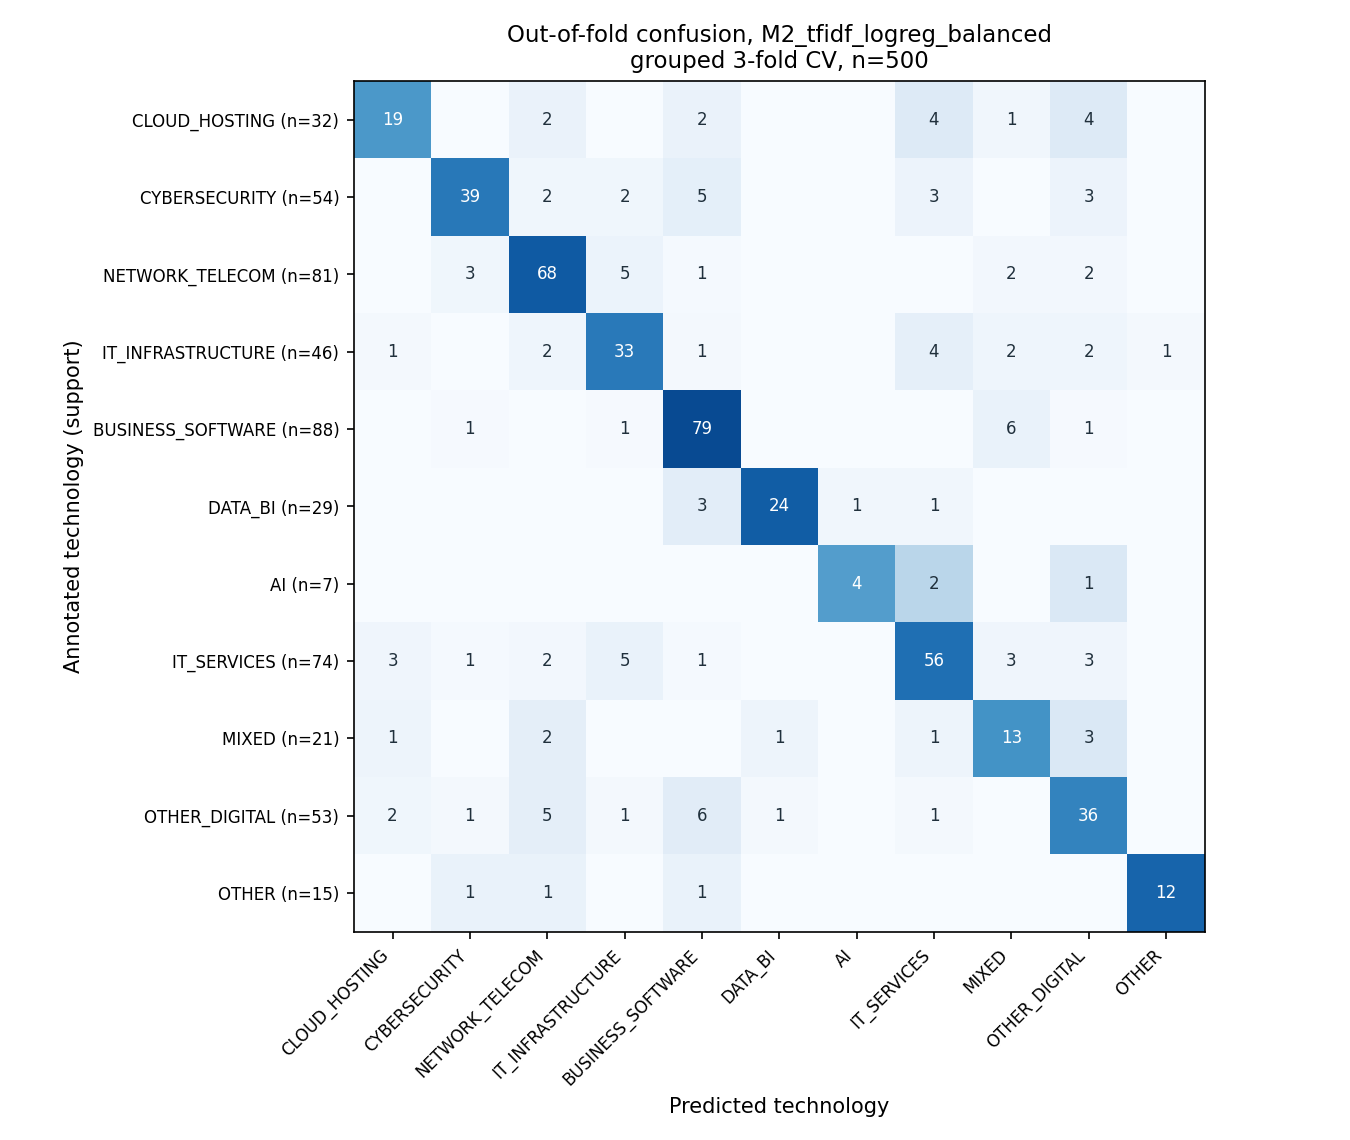
\includegraphics[width=0.85\linewidth]{figures/appE_tech_confusion.png}
\caption{Out-of-fold confusion matrix over the eleven classes. The dominant confusions run along definitional
boundaries --- \texttt{OTHER\_DIGITAL} against \texttt{BUSINESS\_SOFTWARE} and \texttt{NETWORK\_TELECOM},
\texttt{IT\_SERVICES} against \texttt{IT\_INFRASTRUCTURE} --- rather than being spread at random.}
\label{fig:appe-cm}
\end{figure}

\begin{figure}[htbp]
\centering
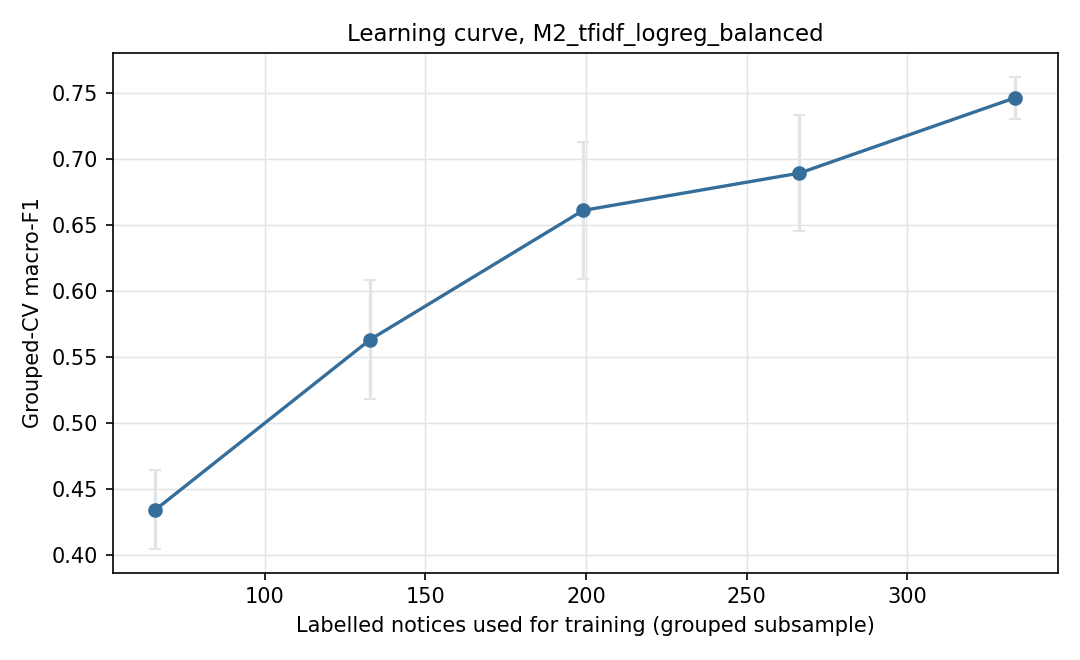
\includegraphics[width=0.72\linewidth]{figures/appE_learning_curve.png}
\caption{Learning curve, subsampling procurement \emph{families} rather than notices. Training F1 sits near
0.99 at every size while validation F1 climbs from 0.434 to 0.747 and has not flattened at $n = 500$. This is
a variance-limited regime: more annotation is the indicated remedy, not more model capacity --- which is the
diagnostic behind the decision not to run a transformer.}
\label{fig:appe-lc}
\end{figure}

\begin{figure}[htbp]
\centering
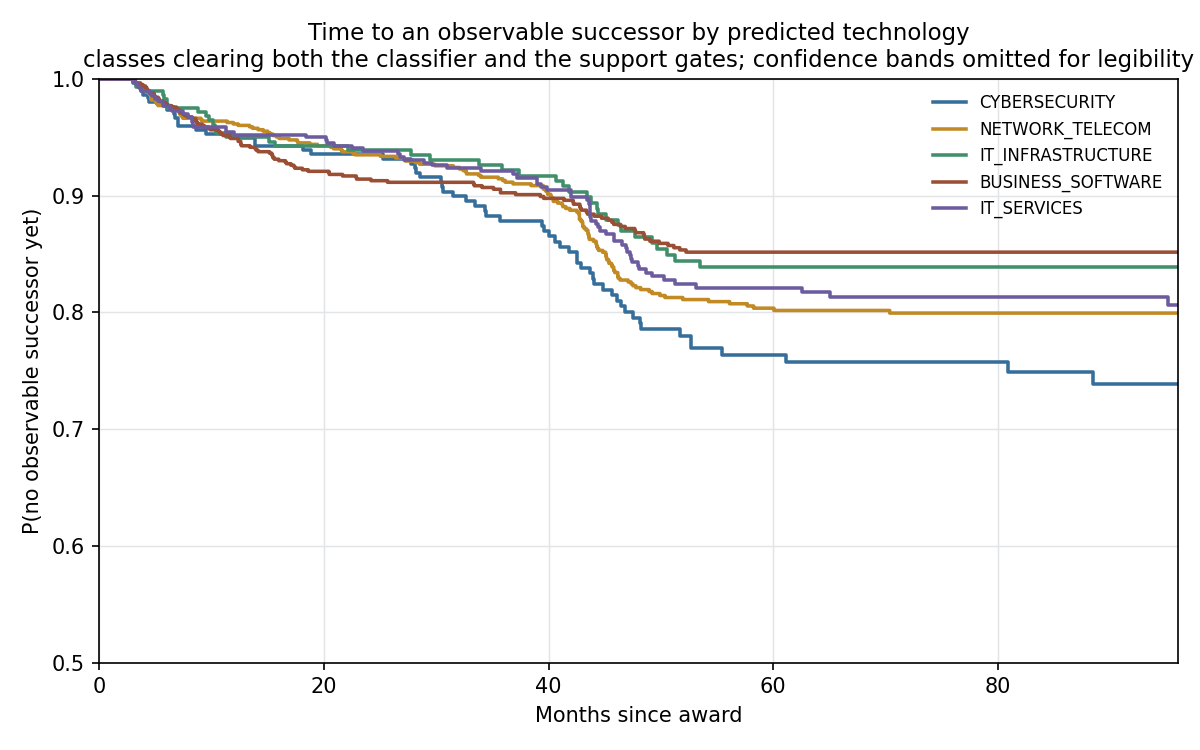
\includegraphics[width=0.78\linewidth]{figures/appE_technology_km.png}
\caption{Kaplan--Meier curves for the five predicted technology classes clearing both Gate A (classifier
quality) and Gate B (downstream statistical support). Confidence bands are omitted for legibility; the axis
starts at 0.5.}
\label{fig:appe-km}
\end{figure}
